\chapter{MALZEME VE YÖNTEM}
\label{ch:malzemeveyontem}

Bu bölümde CloudMon sisteminin geliştirildiği OpenStack deney ortamı, veri toplama altyapısı, sistem mimarisi, log işleme pipeline'ı, özellik mühendisliği, kapasite tahmin modelleri, SHAP analizi ve öneri motoru ayrıntılı olarak açıklanmaktadır.


\section{Sistem Mimarisi}

CloudMon, OpenStack tabanlı özel bulut altyapısının proaktif olarak izlenmesi amacıyla geliştirilmiş altı adımlı bir analiz pipeline'ıdır.
Sistemin genel mimarisi \autoref{fig:mimari}'de gösterilmektedir.

\begin{figure}[htbp]
    \centering
    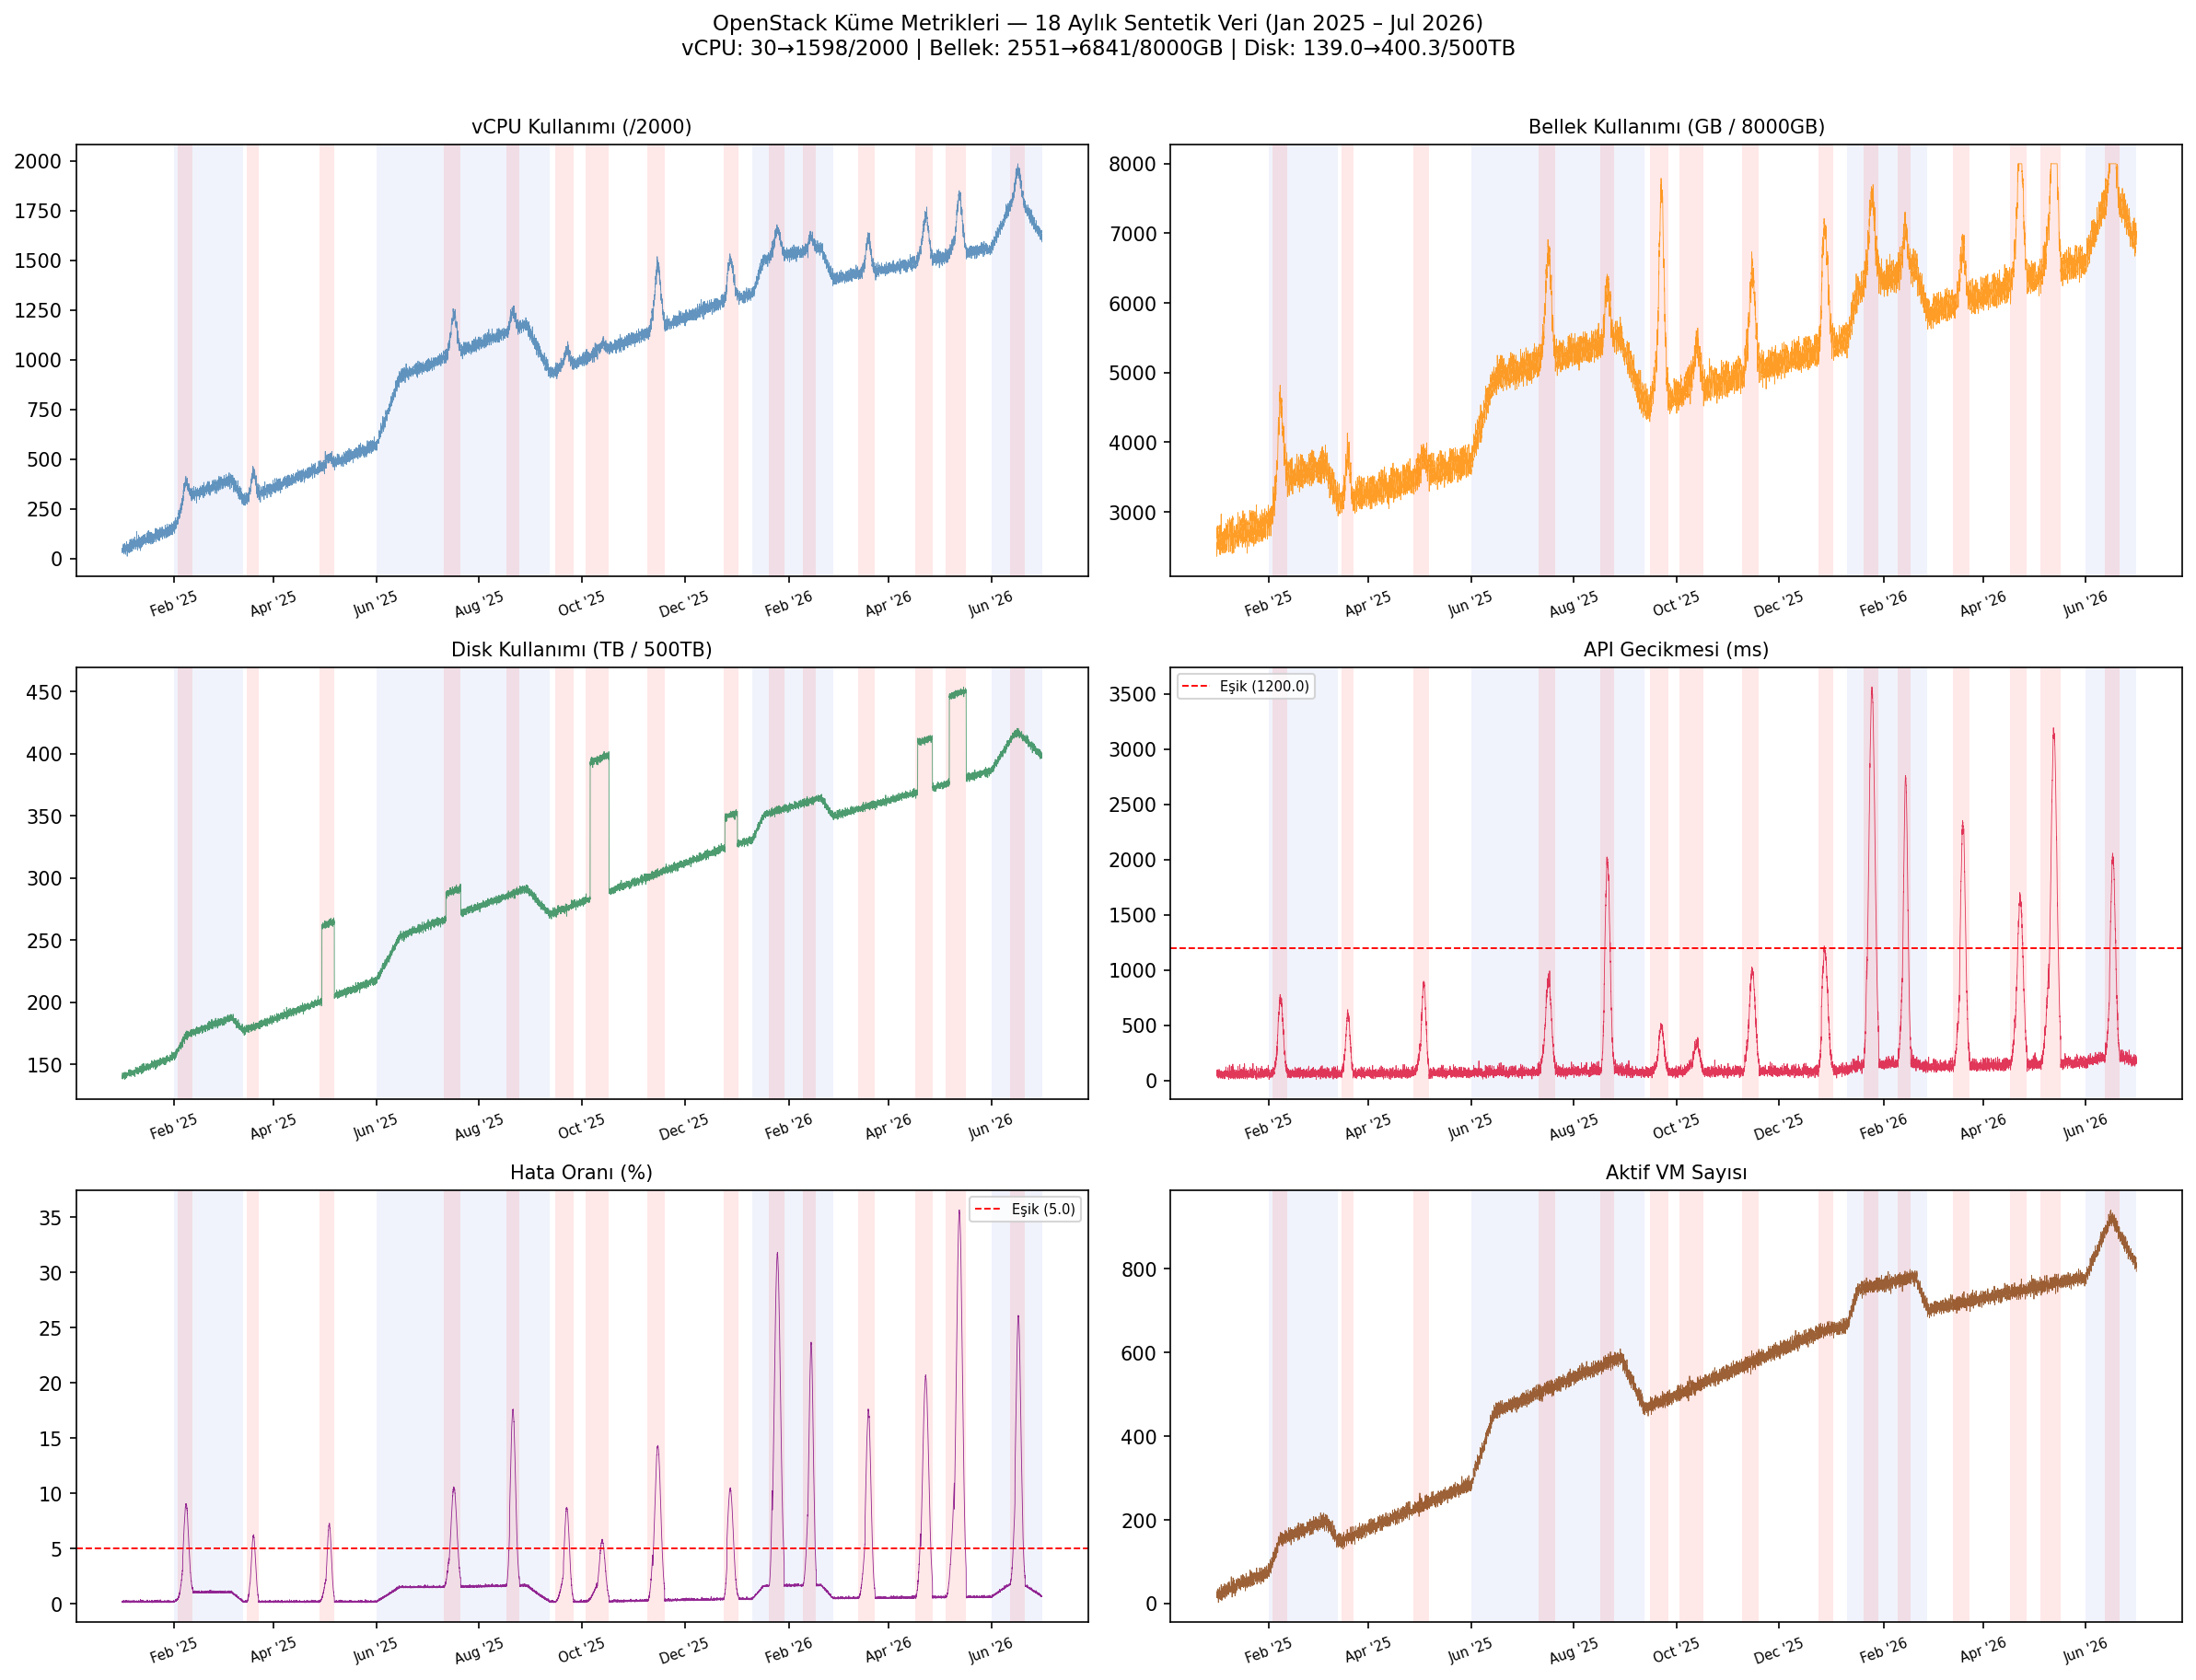
\includegraphics[width=0.95\textwidth]{metrics_overview}
    \caption{CloudMon pipeline'ının genel akışı: veri yükleme, log analizi, özellik mühendisliği, kapasite tahmini, SHAP analizi ve öneri üretimi.}
    \label{fig:mimari}
\end{figure}

Pipeline adımları sırasıyla şunlardır:
\begin{maddelendir}[label=\textbf{Adım \arabic*.}]
    \item \textbf{Veri Yükleme:} Prometheus/Thanos kaynaklı saatlik metrikler (\texttt{metrics.csv}) ve OpenSearch kaynaklı saatlik log özellik tablosu (\texttt{log\_features.csv}) okunur.
    \item \textbf{Log İşleme Hattı:} Dört aşamalı analiz gerçekleştirilir (bkz. \autoref{sec:logpipeline}).
    \item \textbf{Özellik Mühendisliği:} Metrik ve log verilerinden 272 özellik türetilir (bkz. \autoref{sec:ozellik}).
    \item \textbf{Kapasite Tahmini:} Yedi algoritma $\times$ üç kaynak $\times$ iki ufuk = 42 regresyon modeli eğitilir (bkz. \autoref{sec:modeller}).
    \item \textbf{SHAP Analizi:} Her model için özellik atıf değerleri hesaplanır (bkz. \autoref{sec:shap}).
    \item \textbf{Öneri Üretimi:} Kural tabanlı motor ve LLM çıktıları birleştirilerek operasyonel rapor oluşturulur (bkz. \autoref{sec:oneri}).
\end{maddelendir}


\section{Deney Ortamı ve Veri Toplama Altyapısı}
\label{sec:ortam}

\subsection{OpenStack Altyapısı}

CloudMon, TÜBİTAK BİLGEM bünyesinde geliştirilen OpenStack tabanlı özel bulut platformu üzerinde çalıştırılmıştır.
OpenStack, açık kaynak kodlu, modüler bir bulut işletim sistemi olup işlem, depolama ve ağ kaynaklarını API aracılığıyla yazılım katmanından yönetmeye olanak tanımaktadır \autocite{openstack2024}.
Bu çalışmada dört temel OpenStack servisi izleme kapsamına alınmıştır:

\begin{maddelendir}[label=--]
    \item \textbf{Nova (Compute):} Sanal makine yaşam döngüsünü yöneten işlem servisi.
    Kapasite açısından en kritik bileşendir: vCPU ve bellek kaynaklarının tahsisi, VM başlatma/durdurma işlemleri ve zamanlayıcı (scheduler) kararları bu servis tarafından gerçekleştirilmektedir.
    Nova, \texttt{nova-api}, \texttt{nova-compute} ve \texttt{nova-scheduler} alt servislerinden oluşmaktadır; bu alt servisler bağımsız olarak izlenmekte ve servis sağlık skorlarına ayrı ayrı katkı sağlamaktadır.

    \item \textbf{Neutron (Network):} Sanal ağları, alt ağları, yönlendiriciyi ve güvenlik gruplarını yöneten ağ servisidir.
    VM'ler arası ve dış ağ iletişimini sağlar; bant genişliği ve ağ hatası metrikleri bu servis üzerinden izlenmektedir.

    \item \textbf{Cinder (Block Storage):} Sanal makinelere bağlanan kalıcı blok depolama birimlerini yöneten depolama servisidir.
    Disk I/O hatası ve depolama kullanım oranı metrikleri Cinder bileşeninden elde edilmektedir.

    \item \textbf{Keystone (Identity):} Kullanıcı kimlik doğrulama, proje kota yönetimi ve servisler arası yetkilendirmeyi sağlayan kimlik servisidir.
    Kimlik doğrulama hataları ve kota aşımı uyarıları Keystone loglarından türetilmektedir.
\end{maddelendir}

\subsection{Metrik Toplama: Prometheus ve Thanos}

OpenStack servislerinden metrik verisi, Prometheus/Thanos izleme yığını aracılığıyla saatlik aralıklarla toplanmaktadır.
Prometheus, her servisten HTTP endpoint'ler üzerinden metrik kazıma (scraping) yaparak zamanlı metrik dizileri oluşturmaktadır.
Thanos bu yapının üzerine uzun vadeli depolama ve çok bölgeli (multi-region) sorgulama katmanı eklemektedir; bu sayede 18 aylık veri tutarlı biçimde sorgulanabilmektedir.

CloudMon, Prometheus/Thanos'tan saatlik granülarite ile \texttt{metrics.csv} formatında dokuz birincil metriği okumaktadır (\autoref{tab:metrikler}).
Metrik toplama süreci üç aşamadan oluşmaktadır: (i) Prometheus endpoint'lerinden ham verilerin kazınması, (ii) Thanos sorgu katmanı üzerinden saatlik agregasyonun gerçekleştirilmesi ve (iii) CSV formatına dönüştürülerek CloudMon veri dizinine yazılması.

\subsection{Log Toplama: OpenSearch}

OpenStack servis logları OpenSearch platformunda merkezi olarak depolanmaktadır.
Fluentd log iletim aracı, Nova, Neutron, Cinder ve Keystone servislerinin \texttt{/var/log/} çıktılarını gerçek zamanlı olarak OpenSearch endekslerine aktarmaktadır.

CloudMon log işleme için ham log satırlarını değil, önceden belirlenmiş 15 log tipi üzerinden saatlik pencere bazında hesaplanan sayımları kullanmaktadır (\texttt{log\_features.csv}).
Bu yaklaşım iki avantaj sağlamaktadır: birincisi, log hacmine bağlı hesaplama maliyetini sabit ve öngörülebilir kılmak; ikincisi, log ayrıştırma (parsing) adımını CloudMon dışında OpenSearch sorgu katmanında gerçekleştirerek pipeline'a temiz ve yapılandırılmış girdi sağlamak.

Saatlik log özellik tablosu şu şekilde üretilmektedir: her saat dilimi için her log tipi, ilgili OpenSearch endeksinde anahtar kelime eşleşmesiyle sorgulanmakta ve bulunan kayıt sayısı tek bir satıra yazılmaktadır.
Bu işlem \texttt{raw\_logs.csv} içindeki ham log örneklemesiyle desteklenmekte; ön-arıza örüntü çıkarımı (Aşama 4) ham loglar üzerinden çalıştırılmaktadır.

\subsection{Veri Akışı}

\autoref{fig:veriakisi}'de CloudMon'un uçtan uca veri akışı görülmektedir.
OpenStack servisleri → Prometheus/Thanos → \texttt{metrics.csv} hattı metrik verisi sağlarken, OpenStack servisleri → Fluentd → OpenSearch → \texttt{log\_features.csv} hattı log özellik tablosunu üretmektedir.
Her iki kaynak saatlik granülaritede CloudMon ana pipeline'ına beslenmekte; özellik mühendisliği adımında tek bir 272 boyutlu vektöre birleştirilmektedir.

\begin{figure}[htbp]
    \centering
    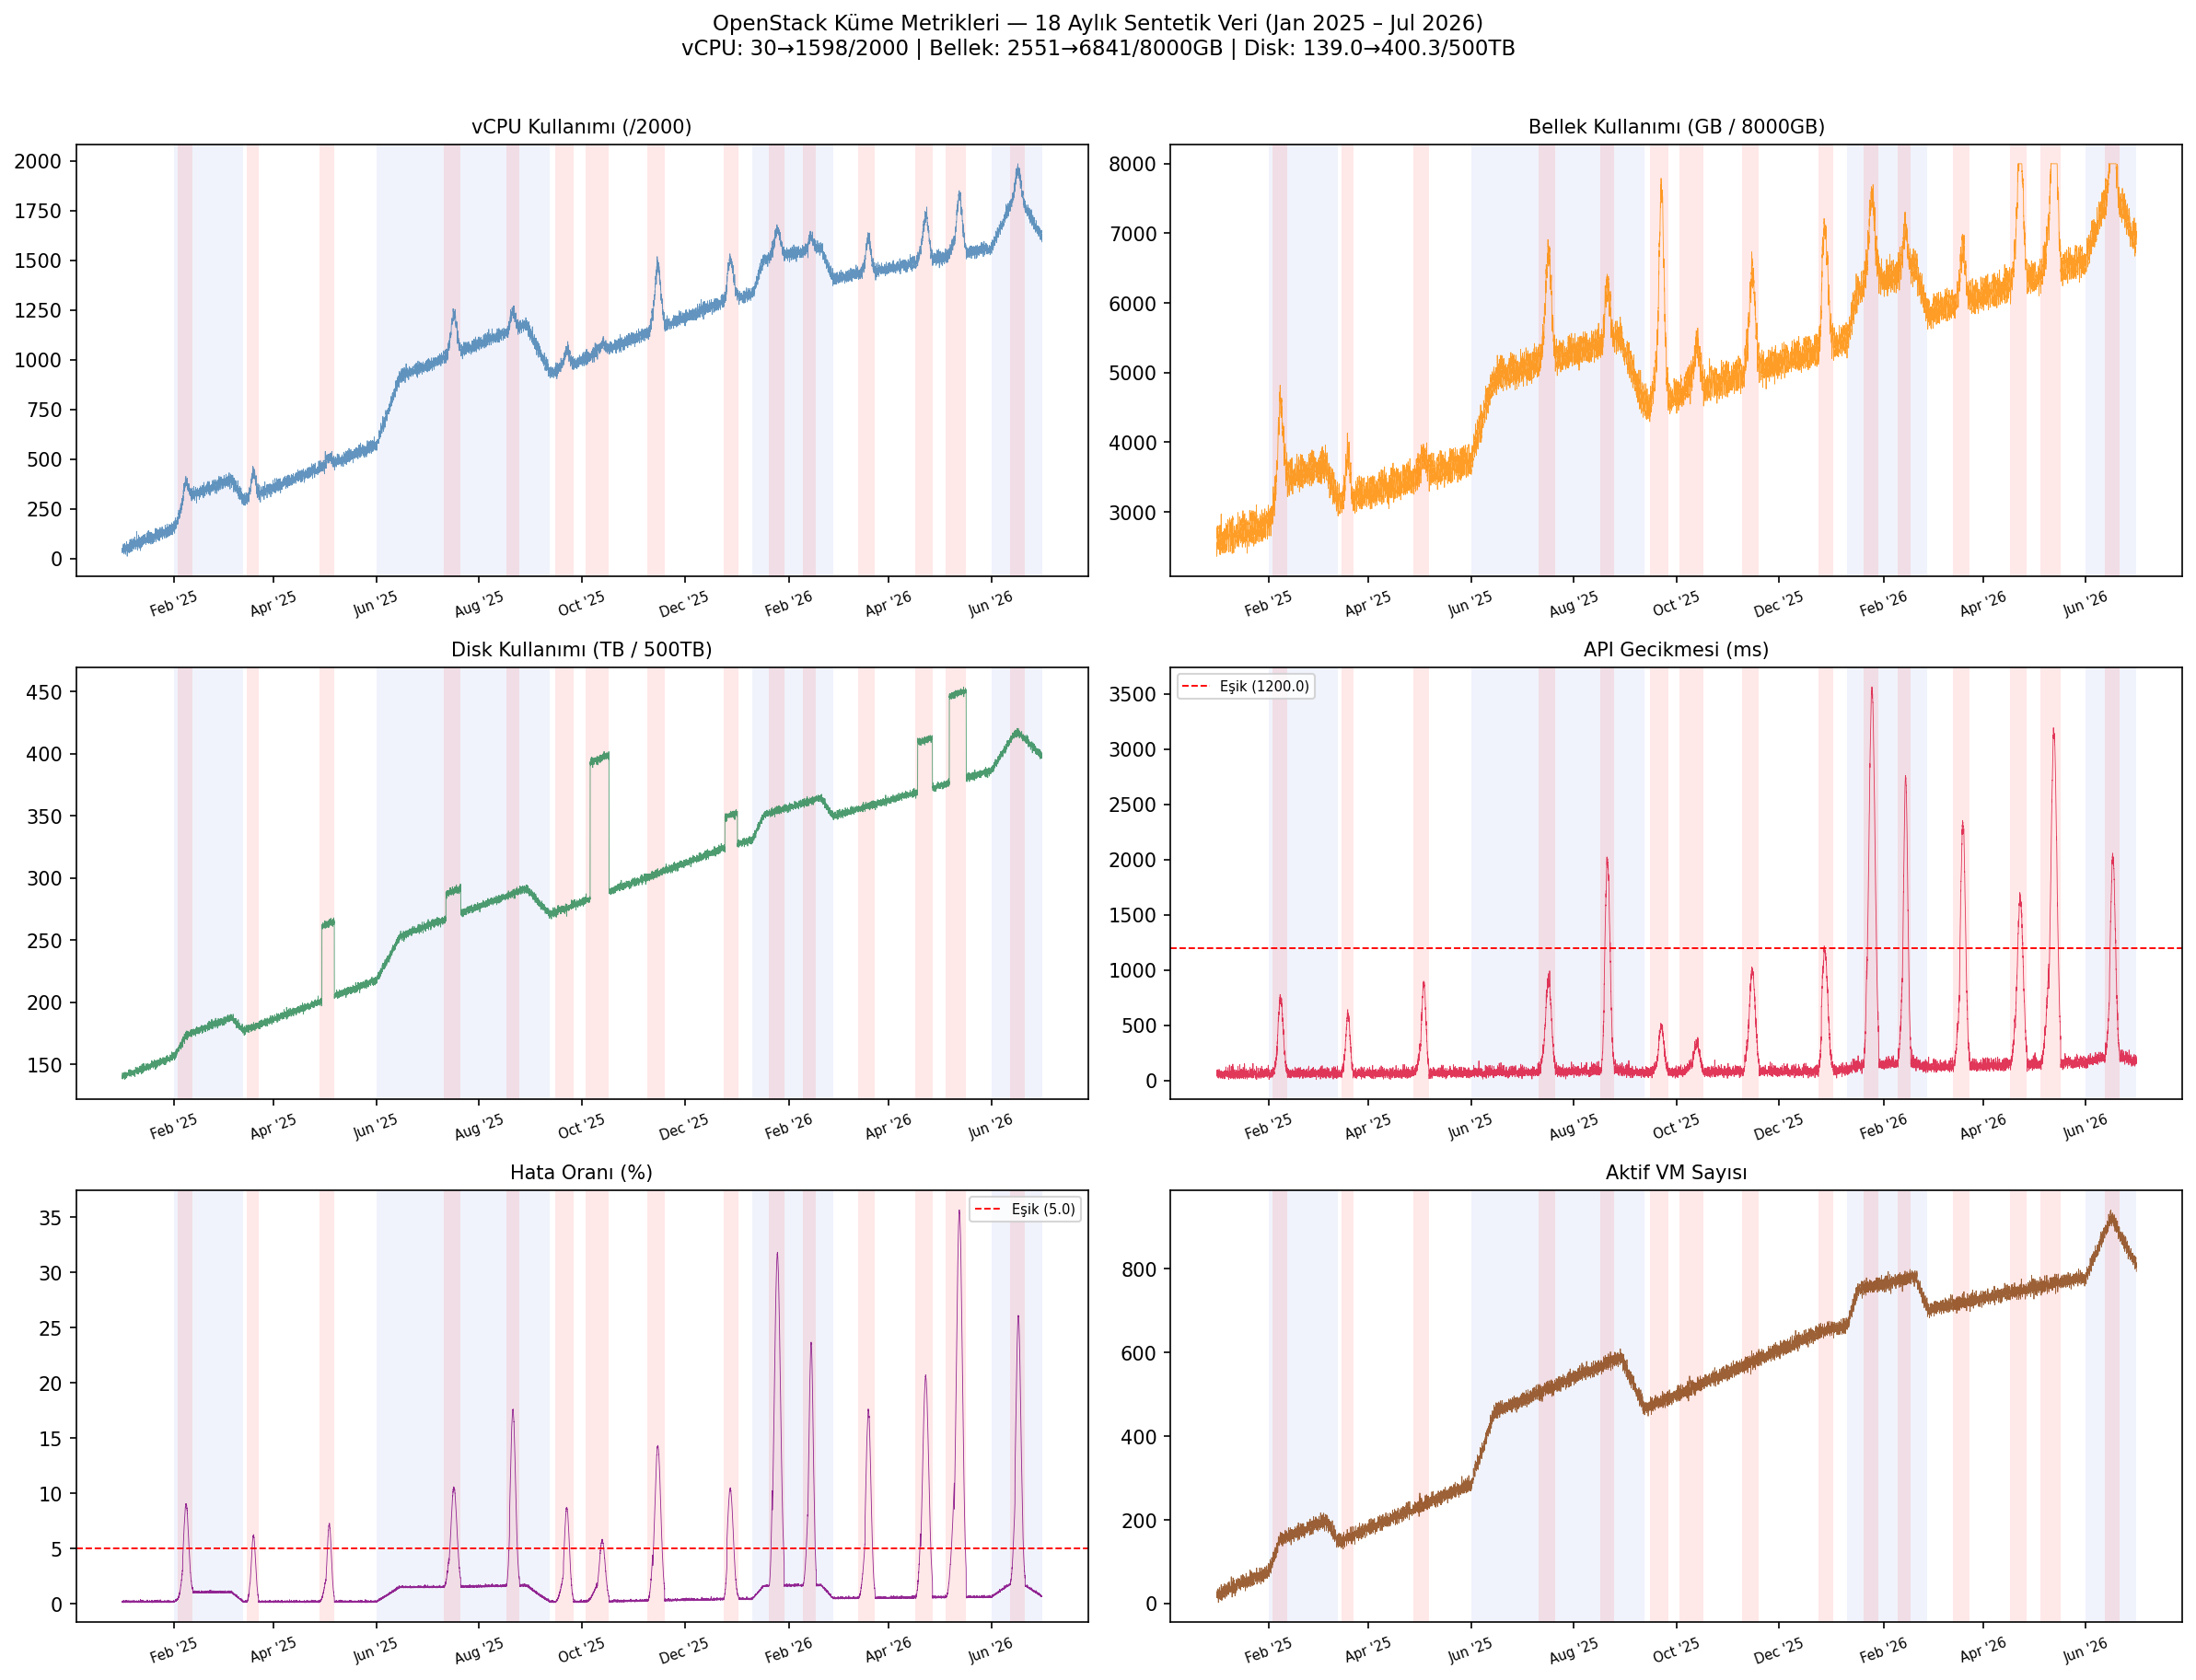
\includegraphics[width=0.92\textwidth]{metrics_overview}
    \caption{CloudMon veri akışı: OpenStack servislerinden metrik (Prometheus/Thanos) ve log (Fluentd/OpenSearch) verilerinin toplanması ve pipeline'a beslenmesi.}
    \label{fig:veriakisi}
\end{figure}


\section{Veri Kümesi}

\subsection{Metrik Verisi}

Metrik verisi, OpenStack Nova (işlem), Cinder (depolama) ve Neutron (ağ) bileşenlerinden Prometheus/Thanos aracılığıyla saatlik aralıklarla toplanmıştır.
Veri kümesi Ocak 2025 -- Temmuz 2026 dönemini kapsayan 18 aylık bir zaman aralığına karşılık gelmekte ve toplam 13.104 saatlik gözlem noktası içermektedir.

Birincil kaynak değişkenleri \autoref{tab:metrikler}'de özetlenmektedir.

\begin{table}[htbp]
    \centering
    \caption{Kullanılan metrik değişkenleri}
    \label{tab:metrikler}
    \begin{tabular}{lll}
        \textbf{Değişken} & \textbf{Açıklama} & \textbf{Birim} \\
        \hline
        \texttt{vcpu\_usage\_percent}   & vCPU tahsis oranı      & \% \\
        \texttt{memory\_usage\_percent} & Bellek kullanım oranı  & \% \\
        \texttt{disk\_usage\_percent}   & Disk kullanım oranı    & \% \\
        \texttt{api\_latency\_ms}       & API yanıt gecikmesi    & ms \\
        \texttt{error\_rate\_percent}   & Hata oranı             & \% \\
        \texttt{network\_in\_mbps}      & Gelen ağ trafiği       & Mbps \\
        \texttt{network\_out\_mbps}     & Giden ağ trafiği       & Mbps \\
        \texttt{api\_requests\_per\_hour} & Saatlik API istek sayısı & adet/saat \\
        \texttt{vm\_count}              & Aktif sanal makine sayısı & adet \\
    \end{tabular}
\end{table}

\subsection{Log Verisi}

Log verisi, OpenSearch'te depolanan OpenStack servis loglarından saatlik pencere bazında sayım olarak türetilmiştir.
Log tipleri iki kategoriye ayrılmaktadır:

\textbf{Hata logları} (8 tip): \texttt{timeout}, \texttt{db\_connection}, \texttt{resource\_exhausted}, \texttt{quota\_exceeded}, \texttt{auth\_failure}, \texttt{network\_error}, \texttt{scheduler\_error}, \texttt{io\_error}.

\textbf{Erken uyarı logları} (7 tip): \texttt{slow\_response}, \texttt{memory\_pressure}, \texttt{connection\_pool\_warn}, \texttt{scheduler\_degradation}, \texttt{quota\_pressure}, \texttt{disk\_io\_degradation}, \texttt{cascade\_indicator}.

Erken uyarı logları hata statüsüne ulaşmamış ancak sistem degradasyonuna işaret eden ön-arıza sinyallerini temsil etmektedir.

\subsection{Eğitim ve Test Bölünmesi}

Zaman serisi veri setinde bilgi sızıntısını (data leakage) önlemek amacıyla sabit kesim noktası yöntemi kullanılmıştır.
Ocak 2025 -- Mart 2026 arası 15 aylık dönem eğitim kümesini, Nisan 2026 -- Haziran 2026 arası 3 aylık dönem ise test kümesini oluşturmaktadır.
Bu bölünme yaklaşık \%83 eğitim -- \%17 test oranına karşılık gelmektedir.


\section{Log İşleme Pipeline'ı}
\label{sec:logpipeline}

Ham log sayımlarından operasyonel içgörülere ulaşmak amacıyla dört aşamalı bir pipeline tasarlanmıştır.
Pipeline çıktısı \autoref{fig:logpipeline}'de görselleştirilmektedir.

\begin{figure}[htbp]
    \centering
    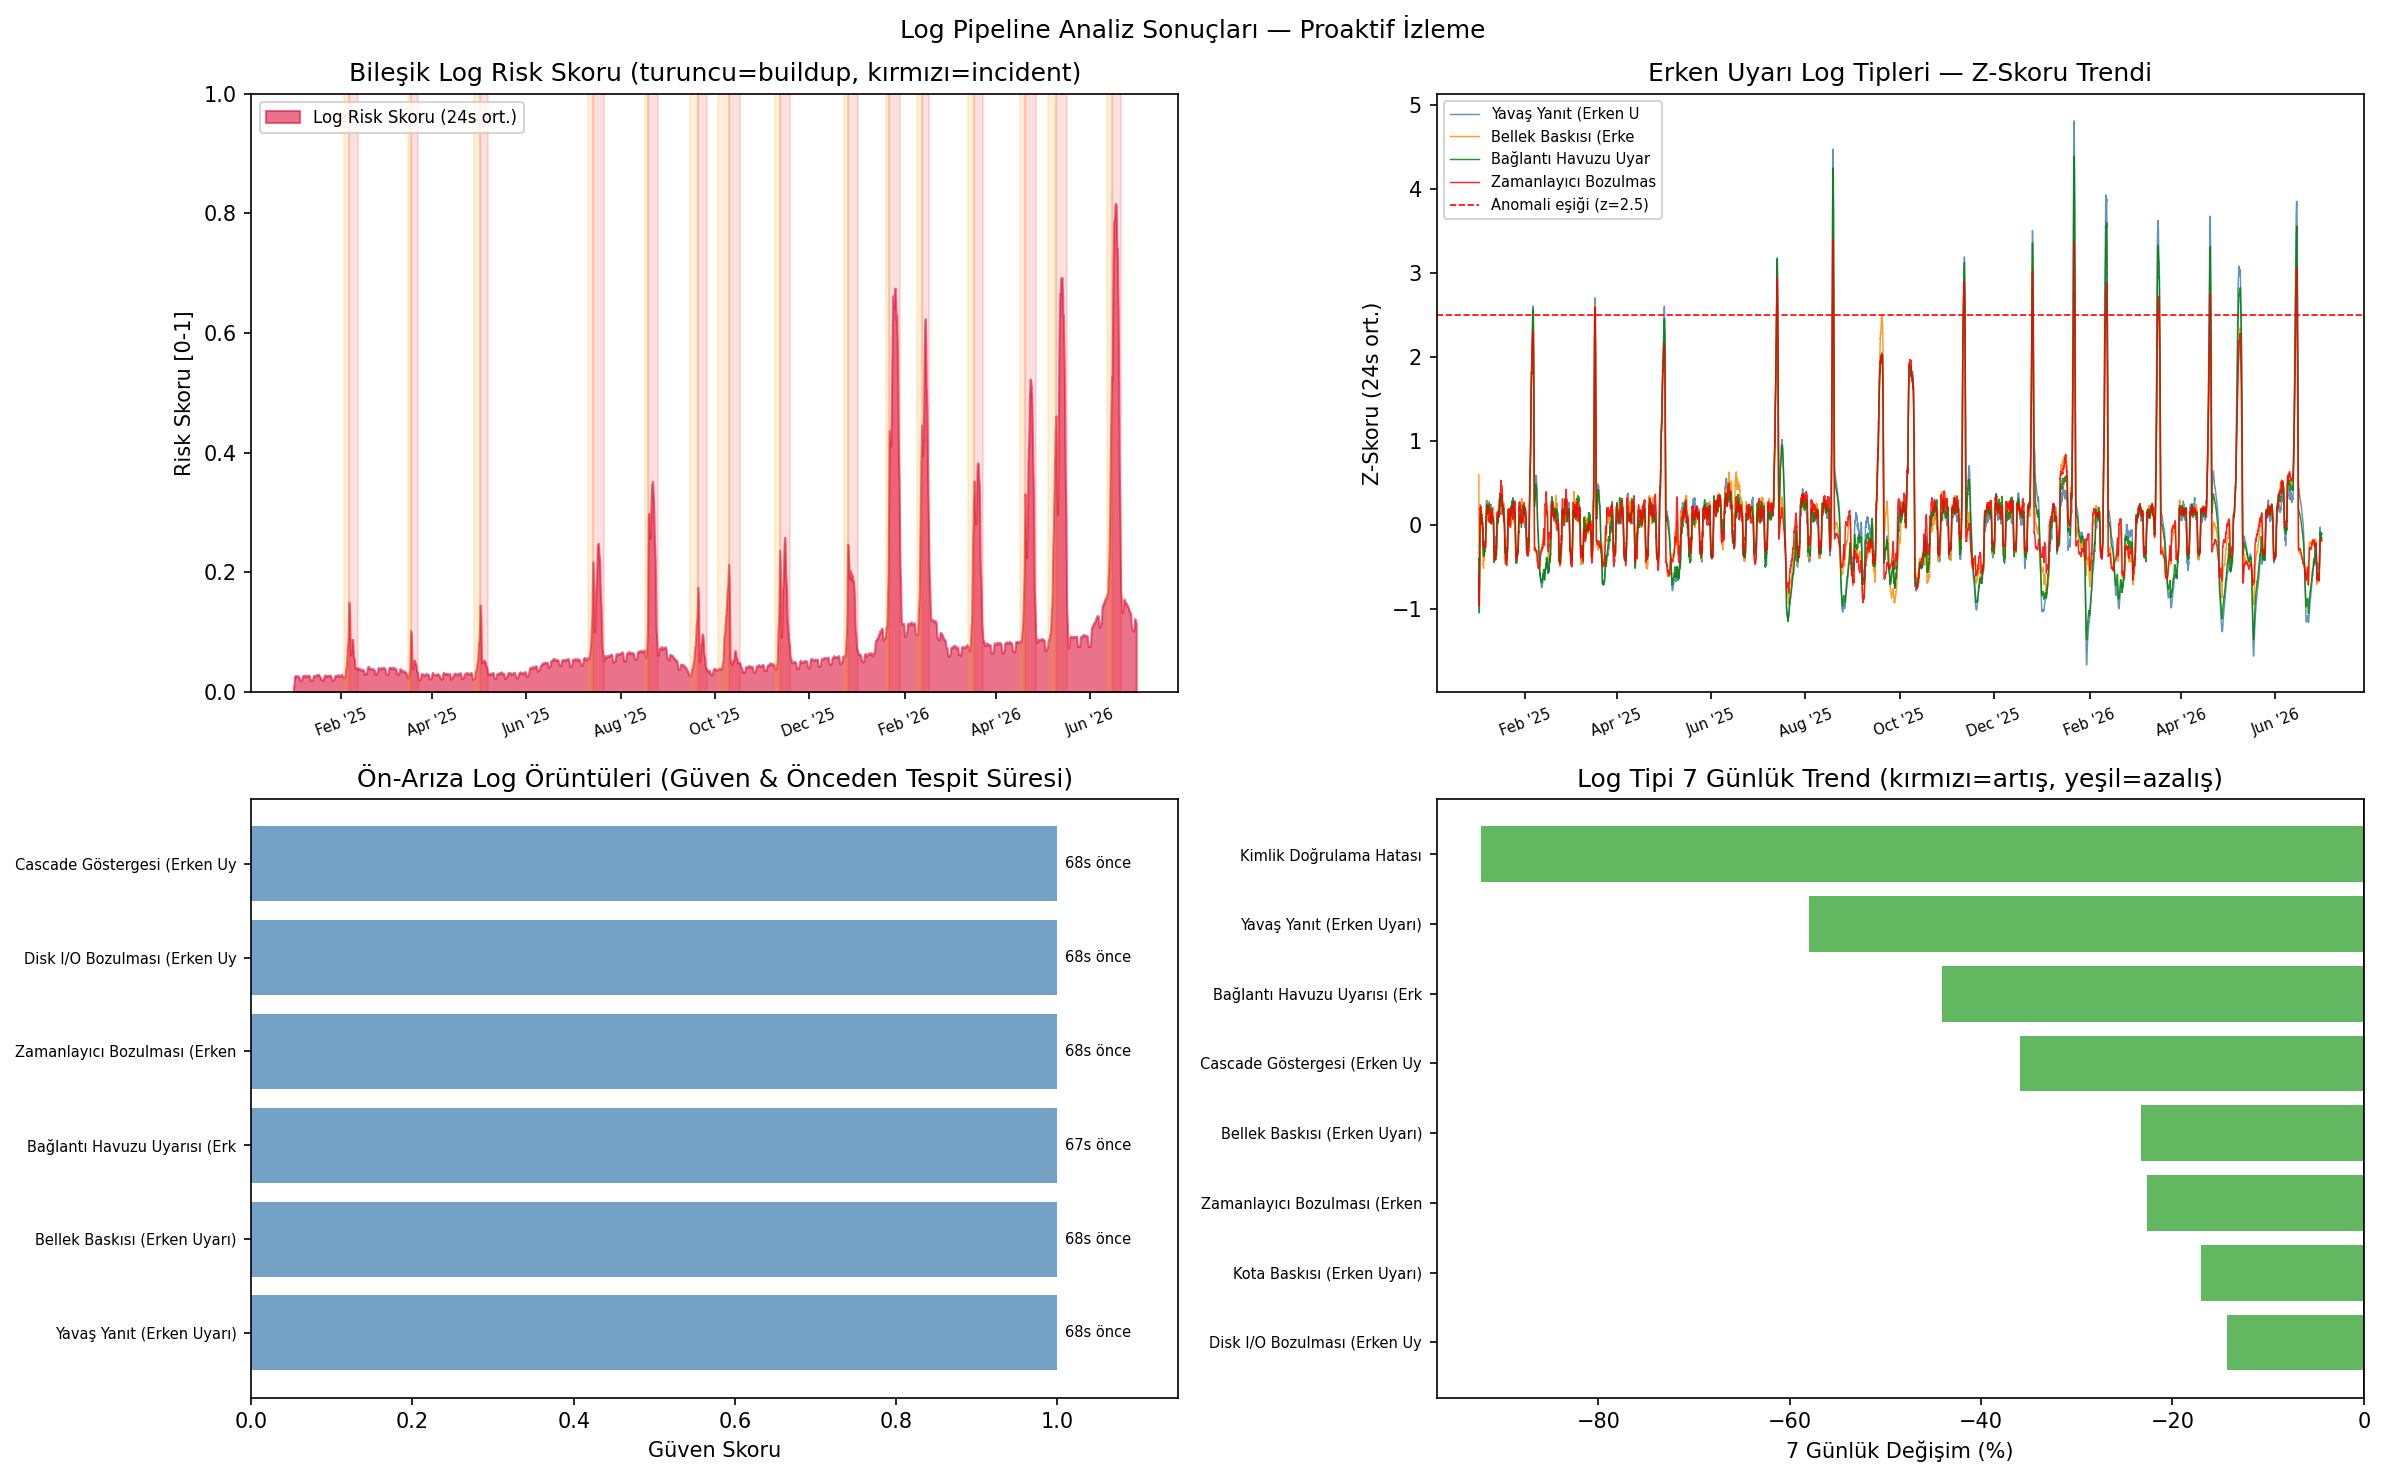
\includegraphics[width=0.90\textwidth]{log_pipeline_analysis}
    \caption{Dört aşamalı log işleme pipeline'ı çıktıları: log trendi, anomali tespiti ve cascade analizi.}
    \label{fig:logpipeline}
\end{figure}

\subsection{Aşama 1 — Ayrıştırma ve Sınıflandırma}

Bu aşamada ham log sayımları Nova, Neutron, Cinder ve Keystone servisleri bazında servis sağlık skorlarına dönüştürülmekte; erken uyarı ve hata logları ayrı ayrı değerlendirilmektedir.

Her servis için normalize hata skoru $s_j \in [0, 1]$ hesaplanmaktadır:
\begin{equation}
    s_j = \min\!\left(\frac{n_j}{q_{99}(n_j) + \epsilon},\; 1\right)
    \label{eq:servis-skor}
\end{equation}
burada $n_j$ servis $j$'nin saatlik hata sayısını, $q_{99}$ \%99'luk dilimi ve $\epsilon$ sıfıra bölmeyi önleyen küçük bir sabiti temsil etmektedir.

Bileşik log risk skoru ise erken uyarı ve hata bileşenlerinin ağırlıklı toplamı olarak tanımlanmaktadır:
\begin{equation}
    r_{\text{log}} = 0{,}4 \cdot s_{\text{uyarı}} + 0{,}6 \cdot s_{\text{hata}}
    \label{eq:log-risk}
\end{equation}
Ağırlıklar; erken uyarı sinyallerinin yüksek hacimli ama düşük öncelikli, hata loglarının ise düşük hacimli ama yüksek öncelikli olduğu kabulünü yansıtmaktadır.
$r_{\text{log}} \in [0, 1]$ aralığında normalize edilmektedir.

Eşiği aşan servisler ($s_j > 0{,}7$: \textit{degraded}; $s_j > 0{,}9$: \textit{critical}) olarak işaretlenmekte ve bu sınıflandırma cascade risk tespitinde (Aşama 3) kullanılmaktadır.

\subsection{Aşama 2 — Zamansal Agregasyon ve Trend Analizi}

Saatlik log sayımlarından 6, 24 ve 72 saatlik hareketli ortalamalar hesaplanmaktadır.
Her log tipi için 7 günlük pencerede z-skor tabanlı trend yönü (\textit{increasing}, \textit{decreasing}, \textit{stable}) belirlenmektedir.

\subsection{Aşama 3 — Anomali Tespiti}

Z-skor eşiği ($\sigma > 2{,}5$) ve ani artış tespiti (spike detection) ile anormal log yoğunlaşmaları belirlenmektedir.
Birden fazla servisin aynı zaman penceresinde degradasyon göstermesi \textit{cascade} riski olarak işaretlenmekte ve zaman damgası kaydedilmektedir.

\subsection{Aşama 4 — Ön-Arıza Örüntü Çıkarımı}

Geçmiş incident'lerin öncesindeki log imzaları bu aşamada çıkarılmaktadır.
Her log tipi için "arızadan kaç saat önce, ne oranda artış gösterdi?" sorusu yanıtlanmaktadır.
Bu örüntüler hem öneri motoruna hem de LLM'e zenginleştirilmiş bağlam olarak beslenmektedir.
Örneğin \textit{slow\_response} log tipi, geçmiş 15 incident'te arızadan ortalama 68 saat önce \%287 artış göstermiştir.


\section{Özellik Mühendisliği}
\label{sec:ozellik}

Metrik ve log verilerinden toplam 272 özellik türetilmektedir.
Bu özellikler altı kategoride sınıflandırılmaktadır:

\begin{table}[htbp]
    \centering
    \caption{Özellik kategorileri ve sayıları}
    \label{tab:ozellikler}
    \begin{tabular}{lll}
        \textbf{Kategori} & \textbf{Tanım} & \textbf{Örnek} \\
        \hline
        Zaman özellikleri      & Saat, gün, hafta, iş günü & \texttt{hour\_of\_day}, \texttt{is\_weekend} \\
        Hareketli ortalama     & 3/6/12/24/168s pencere & \texttt{vcpu\_rmean\_24h} \\
        Hareketli std.         & 3/6/12/24s pencere     & \texttt{vcpu\_rstd\_24h} \\
        Gecikme (lag)          & 1/6/24/48/168s geri    & \texttt{vcpu\_lag\_24h} \\
        Değişim hızı (delta)   & 1/6/24s fark           & \texttt{vcpu\_delta\_6h} \\
        Log hareketli toplamlari & 6/24/72s pencere    & \texttt{slow\_response\_rsum\_72h} \\
    \end{tabular}
\end{table}

Bunlara ek olarak \texttt{early\_warning\_composite} adlı bir bileşik sinyal hesaplanmaktadır.
Bu sinyal, yedi erken uyarı log tipinin saatlik toplamlarını birleştiren ve genel sistem stresini tek bir boyuta indirgeyen bir özet göstergedir.

Hedef değişken her $h \in \{24, 72\}$ saat ufku için üç kaynak ($\hat{y}$: vCPU, Bellek, Disk kullanım yüzdesi) bazında ayrı ayrı oluşturulmaktadır:
\begin{equation}
    \hat{y}_{t+h} = f(\mathbf{x}_t)
\end{equation}
burada $\mathbf{x}_t$ $t$ anındaki 272 boyutlu özellik vektörünü, $f(\cdot)$ ise eğitilen regresyon modelini temsil etmektedir.


\section{Kapasite Tahmin Modelleri}
\label{sec:modeller}

Her (kaynak, ufuk) çifti için yedi farklı algoritma eğitilmekte; böylece $3 \times 2 \times 7 = 42$ model değerlendirilmektedir:

\begin{enumerate}
    \item Doğrusal Regresyon (LR)
    \item Rastgele Orman (RF)
    \item Gradyan Artırmalı Ağaçlar (GBT)
    \item XGBoost (XGB)
    \item LightGBM (LGBM)
    \item CatBoost
    \item Çok Katmanlı Algılayıcı (MLP)
\end{enumerate}

LR ve MLP modelleri için StandardScaler uygulanmaktadır; ağaç tabanlı modeller (RF, GBT, XGB, LGBM, CatBoost) normalizasyon gerektirmemektedir.
Model hiperparametreleri \autoref{tab:hiperparametre}'de özetlenmektedir.

\begin{table}[htbp]
    \centering
    \caption{Kapasite tahmin modelleri hiperparametreleri}
    \label{tab:hiperparametre}
    \begin{tabular}{lll}
        \textbf{Model} & \textbf{Temel Hiperparametreler} & \textbf{Ön İşleme} \\
        \hline
        Doğrusal Regresyon & — (varsayılan) & StandardScaler \\
        Rastgele Orman     & \texttt{n\_est=200, max\_depth=12, min\_leaf=4} & — \\
        Gradyan Artırmalı  & \texttt{n\_est=200, depth=5, lr=0.08, sub=0.85} & — \\
        XGBoost            & \texttt{n\_est=200, depth=5, lr=0.08, sub=0.85} & — \\
        LightGBM           & \texttt{n\_est=200, depth=5, lr=0.08, sub=0.85} & — \\
        CatBoost           & \texttt{iter=200, depth=5, lr=0.08, sub=0.85}   & — \\
        MLP                & \texttt{layers=(128,64), relu, max\_iter=500, early\_stop} & StandardScaler \\
    \end{tabular}
\end{table}

Tüm ağaç tabanlı modellerde \texttt{random\_state=42} sabitlenmiş; tekrarlanabilirlik sağlanmıştır.
MLP'de erken durdurma (early stopping) ile aşırı öğrenme önlenmektedir.

Tüm modeller yinelemeli tahmin (iterative forecasting) stratejisiyle değerlendirilmektedir.
Her test noktasında yalnızca o ana kadar gözlemlenen veri kullanılmakta; böylece gerçek zamanlı operasyonel kullanım koşulları simüle edilmektedir.


\section{SHAP Açıklanabilirlik Analizi}
\label{sec:shap}

\subsection{Neden SHAP?}

Makine öğrenmesi modelleri, özellikle ağaç tabanlı yöntemler, yüksek tahmin başarısı sunmakla birlikte \textit{kara kutu} niteliği taşımaktadır: model neden bu tahmini yaptı sorusunun cevabı doğrudan elde edilememektedir.
Bulut operasyonu bağlamında bu durum ciddi bir güven sorununa yol açmaktadır; bir operatör ``vCPU kullanımı 74 gün içinde eşiği aşacak'' uyarısını aldığında, bu uyarının arkasındaki sinyali anlayamazsa gerekli aksiyonu almakta tereddüt edebilir.

Geleneksel özellik önem yöntemleri bu sorunu yalnızca kısmen çözebilmektedir.
Karar ağaçlarının Gini önem ölçütü yüksek kardinaliteli özelliklere sistematik olarak daha yüksek puan vermekte ve özellikler arası korelasyonu göz ardı etmektedir \autocite{breiman2001}.
Permütasyon önemi ise özelliğin tahmine katkısının yönünü vermemektedir; bir özelliğin yüksek permütasyon skoru tahmini iyileştirdiğini mi yoksa stabilize ettiğini mi gösterdiği belirsiz kalmaktadır.

SHAP (SHapley Additive exPlanations), kooperatif oyun teorisindeki Shapley değerlerini makine öğrenmesine uyarlayan, teorik olarak temellendirilen bir açıklanabilirlik çerçevesidir \autocite{lundberg2017}.
Her özellik için hesaplanan $\phi_i$ değeri şu garantiyi taşımaktadır: tüm özellik atıf değerlerinin toplamı modelin tahmini ile referans değer (eğitim seti ortalaması) arasındaki farka tam olarak eşittir.
Bu toplamlanabilirlik (additivity) özelliği sayesinde SHAP, ``bu özellik tahmini ne kadar ve hangi yönde etkiledi'' sorusunu tutarlı biçimde yanıtlamaktadır \autocite{lundberg2020}.

CloudMon bu çerçeveyi iki temel amaç için kullanmaktadır.
Birincisi, 272 özellikli yüksek boyutlu uzayda hangi metrik ve log özelliklerinin tahmine gerçekten katkı yaptığını saptamak; böylece hibrit özellik uzayının faydası nicel olarak ölçülmektedir.
İkincisi, her kapasite uyarısına ``en etkili özellik: \texttt{vm\_count\_rmean\_24h}'' biçiminde bir açıklama eklemek ve bu açıklamayı LLM katmanına iletmek; böylece hem operatöre hem de dile dayalı öneri motoruna bağlam sağlanmaktadır.

\subsection{Teknik Uygulama}

Her eğitilmiş model için model tipine uygun SHAP açıklayıcısı seçilmektedir: RF, GBT, XGB, LGBM ve CatBoost için TreeSHAP, LR için LinearExplainer, MLP için KernelSHAP kullanılmaktadır \autocite{lundberg2017, lundberg2020}.
Bu seçim, her yöntem için teorik geçerlilik koşullarını karşılamaktadır; TreeSHAP ağaç yapılarını verimli biçimde gezer, LinearExplainer doğrusal modellerde analitik çözüm üretir.

Üç tür görselleştirme üretilmektedir:
\begin{maddelendir}[label=--]
    \item \textbf{Bar grafiği:} tüm test gözlemlerinde ortalama $|\phi_i|$ ile global özellik önem sıralaması.
    \item \textbf{Beeswarm grafiği:} her gözlem için $\phi_i$ değerinin dağılımı ve özellik değeriyle renk kodlaması; hem global hem de yerel örüntüleri görselleştirir.
    \item \textbf{Bağımlılık grafiği:} seçili bir özelliğin değeri ile SHAP katkısı arasındaki ilişki; doğrusal olmayan etkileri ortaya koymaktadır.
\end{maddelendir}

vCPU tahmininde elde edilen bar grafiği \autoref{fig:shap-bar-vcpu}'da verilmektedir.

\begin{figure}[htbp]
    \centering
    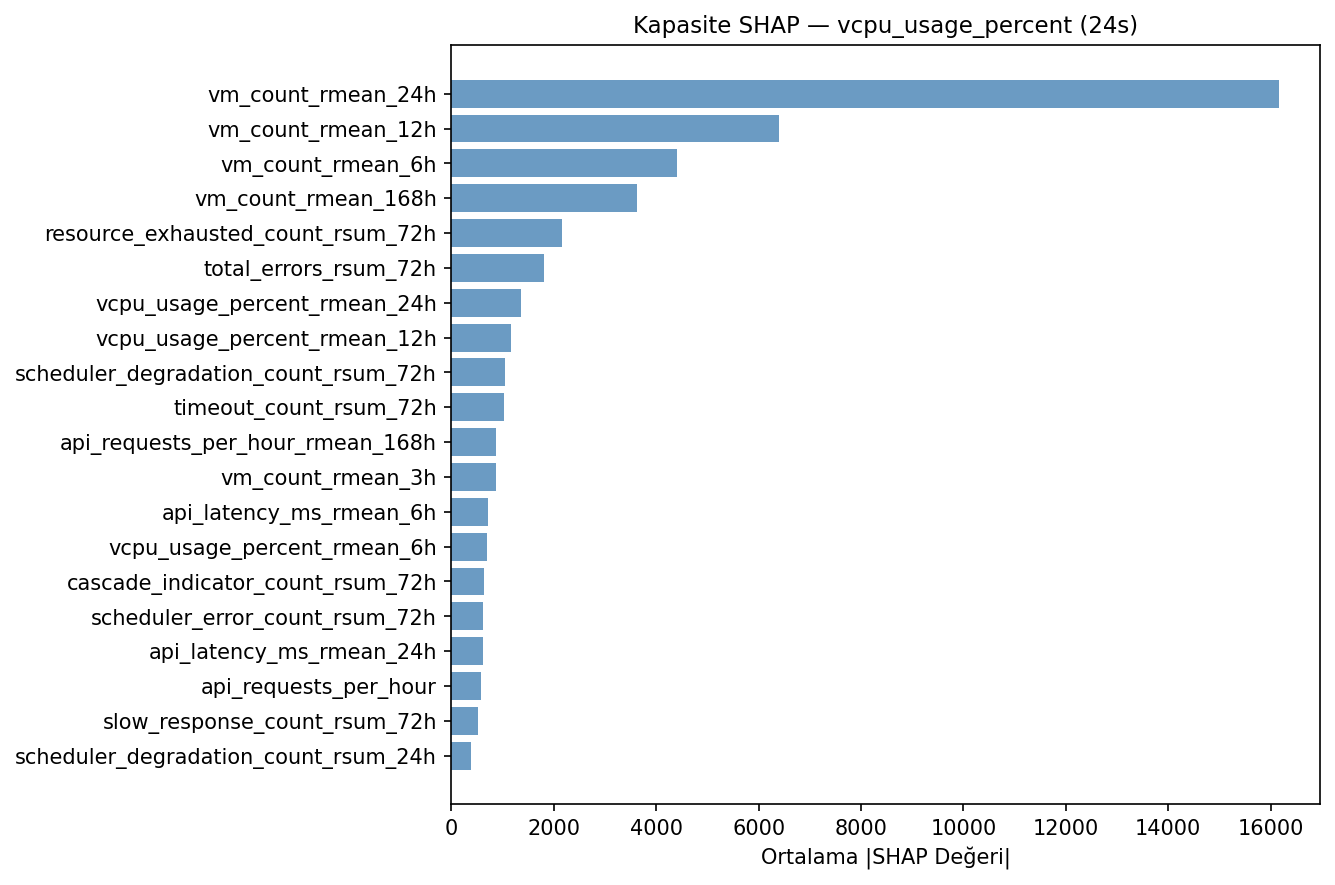
\includegraphics[width=0.85\textwidth]{shap_capacity_bar_vcpu_usage_percent_24h}
    \caption{vCPU 24 saatlik tahmin modeli için SHAP özellik önem sıralaması (ilk 20 özellik).}
    \label{fig:shap-bar-vcpu}
\end{figure}


\section{Öneri Motoru ve LLM Entegrasyonu}
\label{sec:oneri}

\subsection{Neden LLM?}

Kural tabanlı sistemler, eşik aşımlarını ve log anomalilerini güvenilir biçimde tespit eder; ancak bu sinyalleri birleştirerek operatörün ne yapması gerektiğini söyleyemez.
Gerçek bir bulut ortamında aynı anda onlarca uyarı tetiklenebilir: bellek eşiğine yaklaşma, kota aşımı log artışı, zamanlayıcı bozulma ve üç servisin eş zamanlı degradasyonu birbirinden bağımsız alarm olarak göründüğünde, operatör önce hangisine müdahale edeceğine kendi deneyimiyle karar vermek zorunda kalır.

Büyük Dil Modelleri (BDM/LLM), yapılandırılmış bağlam verildiğinde bu sentezi doğal dil akıl yürütmesiyle gerçekleştirebilmektedir.
LLM, hem sayısal verileri (kullanım oranı, z-skoru, tahmini gün sayısı) hem de niteliksel sinyalleri (SHAP sıralaması, ön-arıza örüntüsü, cascade riski) birden okuyan bir uzman gibi davranmakta; bunları önceliklendirilmiş ve gerekçelendirilmiş aksiyon önerilerine dönüştürmektedir \autocite{brown2020, openai2023, anthropic2024}.

CloudMon'da LLM katmanının iki kritik işlevi vardır.
Birincisi, kural motorunun ürettiği ayrı uyarıları tek bir tutarlı operasyonel rapora sentezlemek; ikincisi, SHAP'ın sağladığı ``en etkili özellik'' açıklamasını doğal dil bağlamına taşıyarak operatörün tahminin \textit{neden} yapıldığını anlamasını sağlamaktır.
Bu yaklaşım, CloudMon'u salt bir izleme aracından açıklanabilir ve eyleme dönüştürülebilir bir karar destek sistemine dönüştürmektedir.

\subsection{Neden Zenginleştirilmiş Bağlam?}

LLM performansı, aldığı bağlamın kalitesiyle doğrudan ilişkilidir.
Ham metrik sayıları (``vCPU \%79{,}6, Bellek \%85{,}5'') tek başına bir operasyonel değer taşımaz; modelin bu sayılardan eyleme dönüştürülebilir bir öneri çıkarabilmesi için trendin yönü, beklenen eşik tarihi, log örüntüleri ve SHAP açıklaması gibi bağlam katmanlarına ihtiyacı vardır.
Bu nedenle CloudMon, LLM'e gönderilen istemde şu bilgi katmanlarını birleştirmektedir:

\begin{maddelendir}[label=--]
    \item Kapasite durumu: mevcut kullanım oranı, eşik değeri, trend ve tahmini aşım tarihi
    \item SHAP özellik sıralaması: tahmine en çok katkı yapan metrik veya log tipi (operatörün müdahale noktasını belirlemesi için)
    \item Log anomali özeti: z-skor eşiklerini aşan log tipleri ve yüzdesel artış değerleri
    \item Ön-arıza örüntüsü: geçmiş incident imzalarıyla örtüşen güncel log artışları ve tarihsel öncü süre
    \item Cascade risk bilgisi: eş zamanlı degradasyon gösteren servisler
    \item Servis sağlık durumu: her OpenStack servisinin anlık durum özeti
\end{maddelendir}

\subsection{Kural Tabanlı Katman}

LLM'e iletilmeden önce kural tabanlı motor dört kanaldan uyarı üretmektedir:
\begin{maddelendir}[label=\arabic*.]
    \item \textbf{Kapasite kanalı:} Kapasite modeli tahminleri ve lineer trend analizi birleştirilmekte; tahmini eşik aşım tarihi hesaplanmaktadır. vCPU için $+0{,}275\%$/gün artış trendi ve \%90 eşiği göz önüne alındığında tahmini eşik tarihi çalışma zamanında dinamik olarak belirlenmektedir.
    \item \textbf{Log anomali kanalı:} Z-skor eşiğini ($\sigma > 2{,}5$) aşan log tiplerinde uyarı üretilmektedir.
    \item \textbf{Ön-arıza örüntü kanalı:} Aşama 4'te çıkarılan geçmiş arıza imzalarıyla örtüşen güncel log örüntüleri tespit edilmektedir.
    \item \textbf{Cascade risk kanalı:} Birden fazla servisin eş zamanlı degradasyonu cascade uyarısı olarak raporlanmaktadır.
\end{maddelendir}

\subsection{LLM Katmanı}

Kural tabanlı katmanın çıktıları yukarıda listelenen bağlam katmanlarıyla birleştirilerek yapılandırılmış bir istem oluşturulmaktadır.
Bu istem Claude Sonnet (\texttt{claude-sonnet-4-6}) ve GPT-4o (\texttt{gpt-4o}) modellerine paralel olarak iletilmektedir.
Her iki modelin yanıtı tek bir operasyonel rapora derlenmekte; KRİTİK / UYARI öncelik sıralaması ve servis bazında somut aksiyon önerileri içermektedir.
API anahtarı yapılandırılmadığında sistem, kural tabanlı katmanın çıktılarını doğrudan raporlamakta; LLM sentez katmanı devre dışı kalmaktadır.
